\documentclass{article}
\usepackage[utf8]{inputenc}
\usepackage{fullpage, graphicx, amssymb, amsmath, amsfonts, amsthm, mathtools, physics}
\newcommand{\vectorproj}[2][]{\textrm{proj}_{\vect{\vb*{#1}}}\vect{\vb*{#2}}}
\newcommand{\vect}{\mathbf}


\title{Homework 1}
\author{Manjari Senthilkumar}
\date{18 June 2021}

\begin{document}

\maketitle

\section{Linear Transformation}
\subsection{$\mathbb{E}[\vb*{y}] = \mathbb{E}[A\vb*{x}+b] = A\mathbb{E}[\vb*{x}]+\vb*{b}$}

Since $\vb*{y}$ is a continuous function, the expected value can be calculated as follows:

\begin{align*}
    \mathbb{E}[\vb*{y}] 
        & = \int f(\vb*{y}) \cdot \vb*{y} d\vb*{y}    \\ 
        & = \int f(A\vb*{x}+\vb*{b}) (A\vb*{x} + \vb*{b}) d\vb*{x} \\
    \intertext{Note: since $\vb*{x}$ is the only random variable, the probability density function, $f(A\vb*{x}+ \vb*{b}) = f(\vb*{x})$ and $\mathbb{E}[x] = \int f(\vb*{x}) \cdot \vb*{x} d\vb*{x}$} 
        & = \int f(\vb*{x}) \cdot (A\vb*{x} + \vb*{b}) d\vb*{x} \\
        & = A \int f(\vb*{x}) \cdot \vb*{x} d\vb*{x} + \vb*{b} \int f(\vb*{x})d\vb*{x} \\
        & = A\mathbb{E}[\vb*{x}] + \vb*{b} 
\end{align*}

\subsection{cov$[\vb*{y}] = A {\bf \Sigma} A^T$}
\begin{align*}
    \text{cov}[\vb*{y}] 
        & = \mathbb{E}[(\vb*{y} - \mathbb{E}[\vb*{y}])(\vb*{y} - \mathbb{E}[\vb*{y}])^T] \\
        & = \mathbb{E}[(A\vb*{x} + \vb*{b} - \mathbb{E}[A\vb*{x}+\vb*{b}])  
        (A\vb*{x} + \vb*{b} - \mathbb{E}[A\vb*{x}+\vb*{b}])^T] \\
        & = \mathbb{E}[A(\vb*{x} - \mathbb{E}[\vb*{x}]) 
        (\vb*{x} - \mathbb{E}[\vb*{x}])A^T] \\
        & = A\mathbb{E}[(\vb*{x} - \mathbb{E}[\vb*{x}]) (\vb*{x} - \mathbb{E}[\vb*{x}])]A^T \\
        & = A {\bf \Sigma} A^T
\end{align*}

\section{Linear Regression - Least Squares Solution}
    $\mathcal{D} = \{(0,1),(2,3),(3,6),(4,8)\}$
    \subsection{Cramer's Rule}
    to find the least squares solution to the dataset, we can apply the cramer's rule as follows
    
    \[ 
        m  = \frac{n\sum_{i=1}^n x_i y_i - (\sum_{i=1}^n x_i)(\sum_{i=1}^n y_i)}
        {n \sum_{i=1}^n x_i^2 - (\sum_{i=1}^n x_i)^2}  
    \]
    \[
        b = \frac{(\sum_{i=1}^n x_i^2)(\sum_{i=1}^n y_i) 
                    - (\sum_{i=1}^n x_i)(\sum_{i=1}^n x_i y_i)}
                 {n\sum_{i=1}^n x_i^2 - (\sum_{i=1}^n x_i)^2}
    \]

    \begin{align*}
        \sum_{i=1}^n x_i = 0 + 2 + 3 + 4 & = 9 \\
        \sum_{i=1}^n y_i = 1 + 3 + 6 + 8 & = 18 \\ 
        \sum_{i=1}^n x_i^2 = 0 + 4 + 9 + 16 & = 29 \\ 
        \sum_{i=1}^n x_i y_i = 0 + 6 + 18 + 32 & = 56 
    \end{align*}

    $$m = 62/35 \text{ and } b = 18/35$$

    \subsection{Normal Equations}
    \[ X = \begin{bmatrix}
            1 & 0 \\
            1 & 2 \\
            1 & 3 \\
            1 & 4                 
            \end{bmatrix}\]
    \begin{align*}
        \vb*{\theta*} & = (X^T X)^{-1}X^T \vb*{y} \\
        & = \left(\begin{bmatrix}
            1 & 1 & 1 & 1 \\
            0 & 2 & 3 & 4 
            \end{bmatrix}
            \begin{bmatrix}
            1 & 0 \\
            1 & 2 \\
            1 & 3 \\
            1 & 4                 
            \end{bmatrix}\right)^{-1}
           \begin{bmatrix}
            1 & 1 & 1 & 1 \\
            0 & 2 & 3 & 4 
            \end{bmatrix} 
            \begin{bmatrix} 1 \\ 3 \\ 6 \\ 8 \end{bmatrix} \\
        & = \frac{1}{35} \begin{bmatrix} 18 \\ 62 \end{bmatrix}
    \end{align*}

    \subsection{Graph: least square solution}
        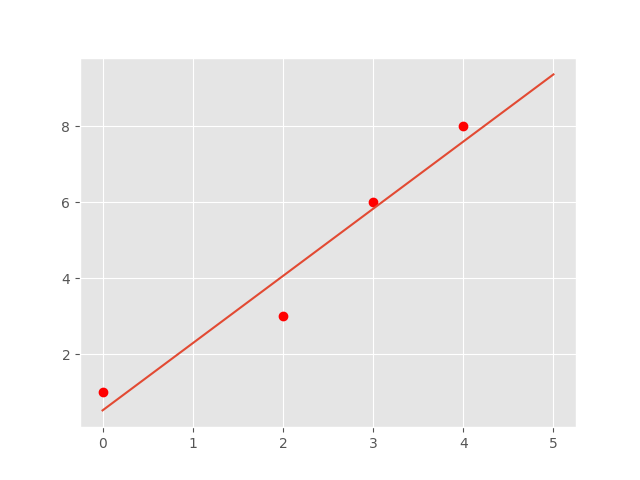
\includegraphics{hw1pr2c.png}
    \subsection{Graph: 100pts with Gaussian Noise}
        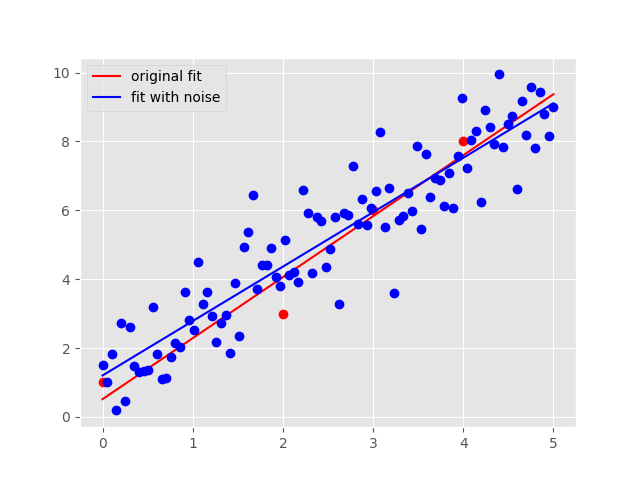
\includegraphics{hw1pr2d.png}
\end{document}
